\chapter{Basic Notions}
\section{ROS2}
ROS2, which stands for robot operating system, is a set of tools and libraries used in robotics applications. Its main objective is to provide an easy and functional way of communicating between processes, which in a real world scenario would each be connected to a functional part of the robot performing some sort of action and interface with other parts when and if necessary. The standard communication principle is the subscribe topic technique.
\subsection{Nodes}
Nodes are the core concept of ROS2, they are each represented by a traditional process and can subscribe and/or publish to topics and services and provide or utilize actions. In a real world example they would logically represent some part of a robot, or a single robot altogether. The ROS2 communication library allows nodes to communicate with each other. The default languages used to define the node's behavior are \texttt{C++} and \texttt{Python3}. Interestingly, it does not matter whether we use one language or the other. ROS2 allows the developer to define the behavior of a node in \texttt{C++} and another in \texttt{Python3} and still have them communicate with each other appropriately.
\subsection{Packages}
Packages contain multiple nodes inside of them. When running a node we must always specify its package. In addition to the nodes behavior specification one can define a launcher which runs multiple nodes following any logic the user may want to follow; a \texttt{XML} and \texttt{CMAKE} file which take care of dependencies and last but not least custom messages, services or actions if one wishes to use them. Although it is a widely followed convention to specify custom interfaces in a separate package.
\subsection{Topics}
Topics are the most used communication tool across nodes in ROS2. They are so fundamental that they could be the only tool used to communicate, even in substitution of actions and services. They are unidirectional and have a many to many relationship, in other words multiple nodes can publish to a single topic and multiple nodes can read the same message at their earliest convenience. A topic is identified using its id, which is used by the publisher to identify in which topic to publish and to the subscriber to decide from which topic to read a message from. The messages sent are used defined based on primitive programming data types such as \texttt{int}, \texttt{char}, \texttt{bool}, etc... Or can also be created including other user defined messages which at their core are primitive data types.   
\subsection{Services}
Services are used whenever a client server architecture is needed, therefore, unlike topics, they are not unidirectional. Here the message does not simply consist of a message containing primitive data types but rather a request message and a response message. As the reader may have already imagined, both the request and response message are user defined messages consisting of primitive data types. One example where one would need services rather than topics would be if we wanted to have one node tell another to do something and to make sure that that action was actually done, which is possible thanks to the response message.
\subsection{Actions}
Actions are very similar to services with the only difference being that they can be interrupted. In addition actions provide multiple response messages during the execution. This allows the issuer to know what percentage of the action has been completed. Like services actions are not essential, for they can be emulated using topics.
\cite{ros2_docs}
\cite{ros2_website}
\section{PDDL}
PDDL stands for planning domain definition language. Like its name suggests it allows the user to define what the world looks like and to feed this definition to a planner which in turn will, whenever possible, output a solution to a problem.
Let us analyze the two main parts of a PDDL problem definition with respect to the 2.1 version, which is the one used by ROS2-BDI.
\subsection{Domain definition}
As anticipated, the domain definition allows the user to define what the world looks like. 
\begin{itemize}
    \item Firstly the \textbf{types} need to be defined. They indicate what kind of object resided in our world. 
    \item \textbf{Predicates} basically are statement about the world which could either be true or false. If a predicate's value is undefined PDDL follows the closed world assumption and assumes everything to be false unless specifically stated otherwise.
    \item \textbf{Actions} indicate which kind of actions can be performed in our world. They are defined by their parameters, which specify the instances in our world which are affected or depend by this action. The duration, which is optional and used only for durative actions, is the time it takes to complete the action. The condition identifies the predicates that must be true for the action to be executed. All conditions must be satisfied at the same time for the action to be considered executable. A condition can be considered \emph{at start}, which means that it needs to be true before the execution even starts; \emph{over all} which means that the condition must be true throughout the execution window and \emph{at end} which is not used in the condition but rather in the effect, which means that the condition will be set to true at the very end of the execution.
    \item \textbf{Effect} states which conditions will be se to true or false at the end (or start if we use the keyword) of the action.
    \item \textbf{Functions} are predicates with real values associated to them. For instance if we wanted to state that the battery of a robot is at 50\% we could say \texttt{battery robot 50}. Needless to say these values can be assigned at the end of an action and can be checked before the execution of one. For example if we wanted to make sure that the robot has enough battery (say 50 \%) at the beginning of the action we could say \texttt{at start (> battery ?robot) 50}. It is also possible to assign a new value to a function or to increase/decrease the current value with a similar syntax.
\end{itemize} 
\subsection{Problem definition} The problem definition's purpose is to define a problem, this is accomplished by:
\begin{itemize}
    \item Detailing which domain this particular problem is referring to.
    \item Listing each object in our world. For instance one could declare the fact that the object whose name shall be \texttt{g} is of type \texttt{robot} by typing \texttt{g - robot}.
    \item Itemizing each true statement at the very beginning of the execution of the world. For example if one wanted to say that the robot \texttt{g} is located at the room \texttt{r} all they would need to write is \texttt{(at g r)}. That is assuming that a predicate \texttt{at} has been previously defined in the domain.
    \item Initialize every function by assigning it a real value.
    \item Specifying the goal. As common sense suggest that is just a list of predicates that we want to be true at the end of the execution of the plan.
\end{itemize}
By doing all of this preliminary work we will be rewarded when we feed our plan to a planner such as Plansys2 because we will be provided with a working plan which has been computed efficiently and automatically.
\cite{pddl_docs}
\section{Webots}
Webots is a 3D robot simulator which is capable of connecting to ROS2 after a little bit of setup. There are countless functionalities which can be used but only the ones that have been used for this project will be described. 
\subsection{World definition} Webots allows its users to define a custom world simply by creating a \texttt{.wbt} file. The idea behind this file is very simple: every object is defined by a reference to a PROTO and the specification of some fields such as the translation (where to position the object), the scale (how much bigger/smaller than default we want this object to be), the color and many many more. A PROTO is a predefined model which specifies every little detail of an object, down to the geometry, physics, contact properties ecc... 
\par
Luckily it gets even easier than that, the user can take advantage of the user interface to create objects and position/modify them as they please. The \texttt{.wbt} file will be modified accordingly and automatically.
\subsection{Robot controller}
Every robot, in addition to initial position and many other properties, has a \texttt{controller} field. This permits the user to define the behavior of the moving parts of the robot, such as the motors. The controller can be defined inside of webots and not use ROS2 communication. Alternatively it can be defined as \texttt{extern} and be controlled by a ROS2 node.
\subsection{Supervisor}
The supervisor is, at its core, a common robot. However, it is capable of much more than a mere robot! In fact it can do whatever it wants. For example it can move objects completely disregarding the physics of the simulation; it can add or remove new objects which can be very helpful for some simulations; it can keep track of the simulation time by reading the \texttt{clock} topic. Being a robot it has a controller, which can very conveniently be a ROS2 node.
\cite{webots_docs}
\section{ROS2-BDI}
As anticipated in the introduction the ROS2-BDI framework comes in two flavors: the offline version and the online version. Their difference is not limited to the way they operate but down to the architectural level. If we wanted to be more precise we should say that there are three versions: the offline version with Plansys2 and the modified version of JAVAFF and the online version with the extension to JAVAFF. Only the first and the latter will be described in the following pages as they were the one used to create the project.
\subsection{Offline ROS2-BDI}
As a reminder, the objective of this design is to have a multi agent framework leveraging all the ROS2 tools and libraries, all while following a BDI based philosophy. Furthermore an automatic planner, Plansys2 in this case, is used to automatically create and execute plans.  

Firstly we shall briefly introduce the architecture of Plansys2 and finally the ROS2-BDI framework built upon it will be presented. 
\subsubsection{Plansys2} Plansys2 is an application whose goal is to compute and execute plans automatically following the PDDL syntax. In short it is able to output a valid plan and to execute it given a pddl domain and a pddl problem.
\par
Since it is built on top of ROS2 its core functionalities are implemented using ROS2 nodes. These core nodes are the executor, the planner, the domain expert and the problem expert. Let us briefly explore these nodes purpose's and interconnections.
\begin{itemize}
    \item The \textbf{executor}, as the name suggests, executes the plan received from the planner. It is connected to each action executor of the client application. Whenever the plan dictates it, it sends an action message to the correspondent client action executor. Furthermore, the executor can be used to modify and cancel the plan via specific ROS2 messages.
    \item The \textbf{planner} communicates via ROS2 services with the domain expert and the problem expert. Basically it looks at the PDDL domain it gets from the domain expert and the PDDL problem it gets from the problem expert and tries to come up with a plan using efficient and reliable algorithms.
    \item The \textbf{domain expert} is basically just a node which forwards the PDDL domain to the planner and gets it from the client application. Unfortunately the domain will always remain the same as Plansys2 does not allow any tempering of it during the execution.
    \item The \textbf{problem expert} is very similar to the domain expert in the sense that it is a node containing the current PDDL problem. However, contrary to the domain it does provide API calls which allow to modify the predicates and functions or to modify/add/cancel the current goal. 
\end{itemize}
\cite{plansys2_docs}
\subsubsection{Architecture} Here is the proposed ROS2-BDI architecture, taken from the official paper.
\begin{figure}[H]
\centering
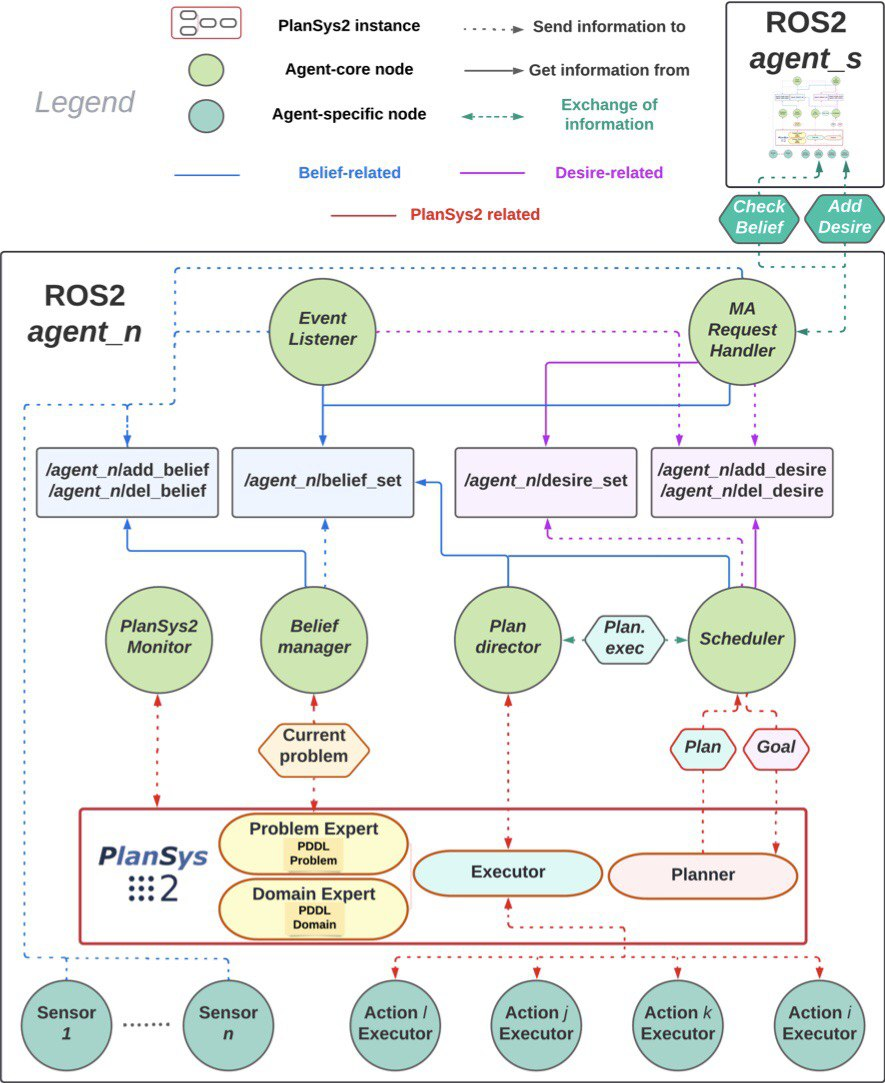
\includegraphics[scale=0.4]{images/offline_architecture.jpg}
\caption{The proposed ROS2-BDI, taken from the official paper}
\end{figure}
It is important to note that all the circles are ROS2 nodes while the rectangles are ROS2 topics. The nodes contained inside the red rectangle compose the Plansys2 instance, every running agent will have its own Plansys2 instance
\par
Let us now shortly go through all the different components that form the ROS2-BDI framework. But before that it is key to differentiate between the different type of nodes in the figure. All the light blue nodes are client application specific and will be different from scenario to scenario. As already mentioned, The red rectangle is the Plansys2 instance and the green nodes are the core nodes of the ROS2-BDI architecture. Everything else is a set of topics with the objective to make the different parts communicate with each other.
\begin{itemize}
    \item \textbf{Plansys2}'s main body is exactly the same way it was described before. It is connected to the client's application action executors and communicates with the core nodes.
    \item The \textbf{sensors} basically look at what is going on in the world and send messages to the topics \texttt{agent\_id/add\_belief} and \texttt{agent\_id/del\_belief} whenever a change occurs. For instance we could have a sensor controlling whether a waypoint is accessible or not. Each and every time the conditions change (i.e. the waypoints switches its state from inaccessible to accessible or vice versa) a message is sent indicating that the belief that the waypoint is accessible needs to be removed or added. It is important to note that the concept of belief is strongly correlated to that of a predicate or function. In fact the belief that the waypoint is accessible is the same as saying that the predicate which indicates that it is is true.
    \item The action executors, like the sensors, are client application dependent. They just wait for an action message to trigger their execution.
    \item The \textbf{Plansys2 monitor}, like its name suggests, continuously exchanges information via ROS2 services with the Plansys2 module to make sure that everything is in working order.
    \item The \textbf{belief manager} has a very basic job, that is to handle request of insertion and deletion of beliefs and to perpetually publish the current beliefs to the \texttt{agent\_id/belief\_set} in order to always have a valid reference. Furthermore, it communicates with the problem expert to make sure that the predicates and functions of the PDDL problem are always up to date. This is an important step that cannot be skipped as the syntax to express a belief differs from that to express a predicate or function.
    \item The \textbf{plan director} basically handles the execution of the plan by initiating it and aborting it if and when necessary.
    \item The \textbf{scheduler} performs a similar job to the belief manager, with the only difference being that it manages the desire set rather than the belief set. In addition to that it decides which plan received from the Plansys2 module to execute and when to abort it or consider it done. 
    \item The \textbf{Event listener} allows to dynamically alter the current state of the world based on the information it receives from the sensors and some rules defined by the programmer. These predefined rules are called reactive rules. For example if we had a world in which the objective is to pick up trash we could, using the reactive rules and the services offered by the request handler, push the desire to retrieve the litter automatically. Obviously these processes are very handy when dealing with dynamic environments where condition change repeatedly.
    \item the \textbf{Multi agent request handler} just forwards the requests from addition and deletion of beliefs and desires.
\end{itemize}
How to practically put ROS2-BDI to use will be clearer in later chapters, for the time being it is enough to have a general idea of how it works.
\cite{ros2_bdi_offline_article}
\cite{ros2_bdi_docs}
\cite{devis_thesis}
\cite{ros2_bdi_offline_demonstration}
\subsection{Online ROS2-BDI} The online version has a lot of similarities to the offline counterpart, both when it comes to the general idea and down to the implementation and means of utilization. 
\par
The main difference in behavior is that the newer online approach start executing a plan even if it is partially created and never stops rescheduling in case new opportunities to fulfill additional desires or to terminate  the execution earlier arise.
\par 
The implementation of the new framework is quite similar in the general structure since it is built upon the offline version as an extension to it. The main differences are the mechanisms which allow to effectuate the new properties and in the planner itself. The planner of choice is a modified version of JAVAFF which has been named OJFF. 
\par 
Since it is possible to switch from the offline version to the online version just by changing some parameters in the launch file the architecture will not be presented as it is extremely similar from a practical point of view.
\subsubsection{OJFF} OJFF is a PDDL 2.1 compliant planner built on top of the JAVAFF planner which allows to follow the properties presented above. The main difference lies in the way the search for a solution is conducted. 
\par
Traditional solution finding algorithms such as the one used by Plansys2 uninterruptedly expand on the search space by adding valid actions at the end of it, all this whilst following well known searching algorithms such as A* and heuristics. This is repeated until exhaustion of the search space or a solution is found. 
\par
On the other hand, OJFF uses another algorithm which differs in the way the search is expanded (it stretches the search from the previous search node until a condition, such as goal reached or maximum depth increment, is met). On top of that it returns the most promising partial solution at the end of each iteration.
\subsubsection{Additional properties needed to make use of temporal planning} Naturally one of these properties is the modified searching algorithm already presented that looks for a solution.
\par
In addition to that a way to forecast the failure of the plan, to improve the solution whenever possible and to revise the goal are necessary. In essence \emph{plan failure forecasting} consists in continually simulating the current plan to check whether it is going to fail or not. In case it does indeed fail, a new plan search which starts from the last committed state is activated. The framework also implements \emph{goal revision} which is the property that allows the planner to try to merge two or more desires in a unique plan whenever possible and more convenient than fulfilling the desires sequentially. Last but not least it adopts a \emph{solution improvement} mechanism which basically means that it tries to make the solution shorter in terms of time whenever possible. That may happen quite often as the framework uses two different algorithm to find a simulation simultaneously. One is quick but usually finds long solutions while the other is slow (with regard to the time it takes to output a valid plan that is) but finds better solutions.
\cite{alex_thesis}
\cite{javaff_repo}
\cite{ojff_repo}
\newpage
